\documentclass{standalone}
\usepackage{tikz}
\usetikzlibrary{patterns, positioning}


\begin{document}
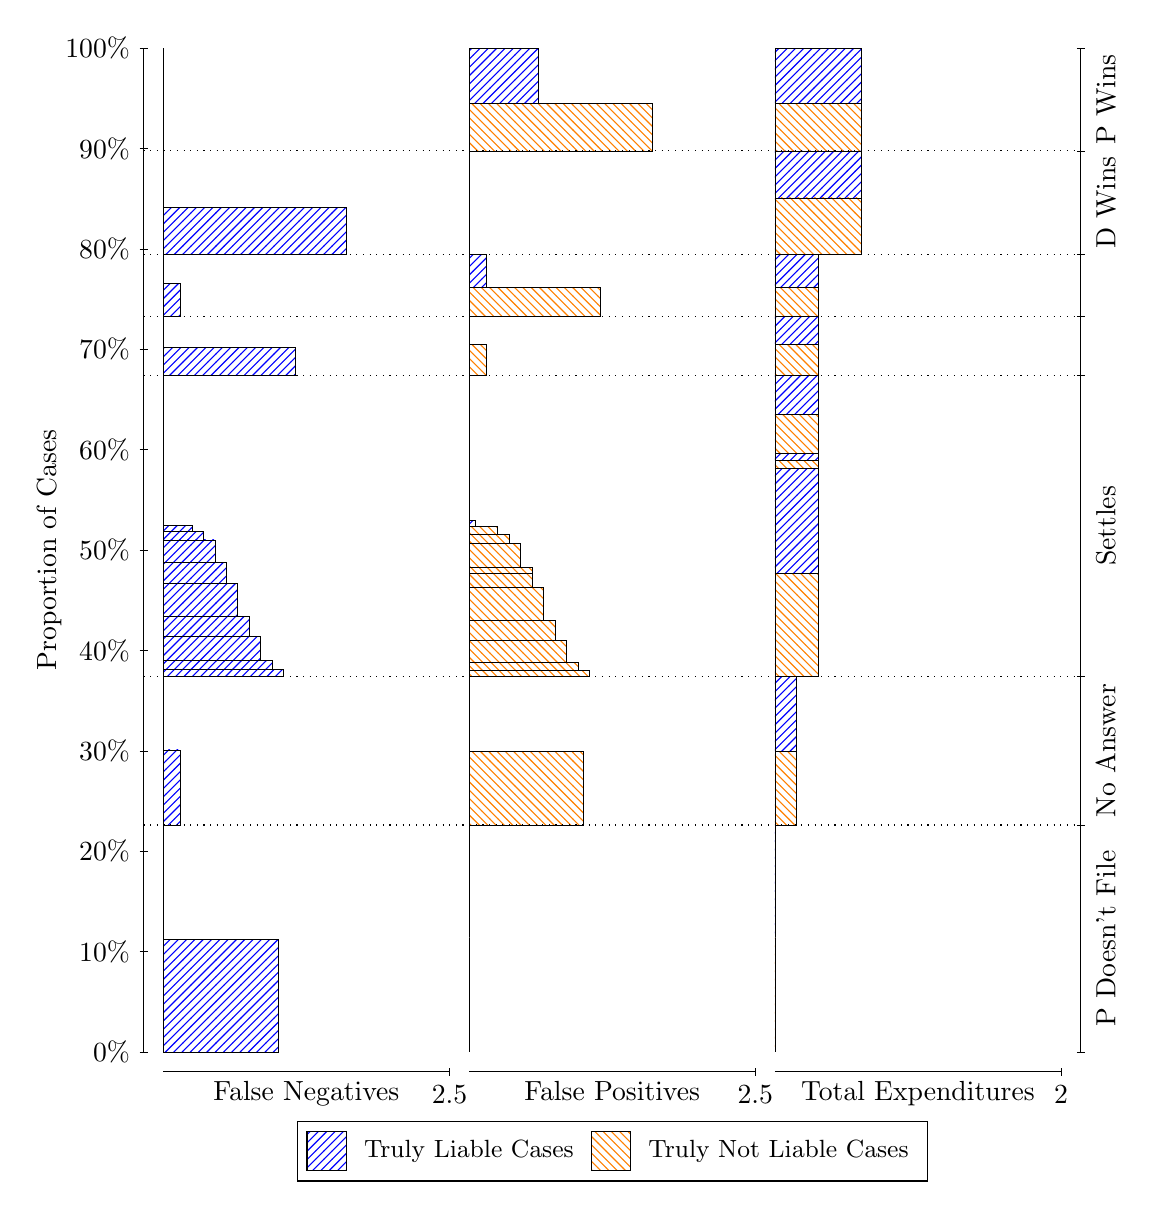
\begin{tikzpicture}
\draw[black, very thin] (1.5,1.75) -- (1.5,14.5);
\node[rotate=90, text=black, anchor=center] at (0.3, 8.125) {Proportion of Cases};
\draw[black, very thin] (1.45,1.75) -- (1.55,1.75);
\node[text=black, anchor=east] at (1.45, 1.75) {0\%};
\draw[black, very thin] (1.45,3.025) -- (1.55,3.025);
\node[text=black, anchor=east] at (1.45, 3.025) {10\%};
\draw[black, very thin] (1.45,4.3) -- (1.55,4.3);
\node[text=black, anchor=east] at (1.45, 4.3) {20\%};
\draw[black, very thin] (1.45,5.575) -- (1.55,5.575);
\node[text=black, anchor=east] at (1.45, 5.575) {30\%};
\draw[black, very thin] (1.45,6.85) -- (1.55,6.85);
\node[text=black, anchor=east] at (1.45, 6.85) {40\%};
\draw[black, very thin] (1.45,8.125) -- (1.55,8.125);
\node[text=black, anchor=east] at (1.45, 8.125) {50\%};
\draw[black, very thin] (1.45,9.4) -- (1.55,9.4);
\node[text=black, anchor=east] at (1.45, 9.4) {60\%};
\draw[black, very thin] (1.45,10.675) -- (1.55,10.675);
\node[text=black, anchor=east] at (1.45, 10.675) {70\%};
\draw[black, very thin] (1.45,11.95) -- (1.55,11.95);
\node[text=black, anchor=east] at (1.45, 11.95) {80\%};
\draw[black, very thin] (1.45,13.225) -- (1.55,13.225);
\node[text=black, anchor=east] at (1.45, 13.225) {90\%};
\draw[black, very thin] (1.45,14.5) -- (1.55,14.5);
\node[text=black, anchor=east] at (1.45, 14.5) {100\%};

\draw[black, very thin] (13.4,1.75) -- (13.4,14.5);
\draw[black, very thin] (13.35,1.75) -- (13.45,1.75);
\node[anchor=west] at (13.35, 1.75) {};
\draw[black, very thin] (13.35,4.6327) -- (13.45,4.6327);
\node[anchor=west] at (13.35, 4.6327) {};
\draw[black, very thin] (13.35,6.5195) -- (13.45,6.5195);
\node[anchor=west] at (13.35, 6.5195) {};
\draw[black, very thin] (13.35,10.343) -- (13.45,10.343);
\node[anchor=west] at (13.35, 10.343) {};
\draw[black, very thin] (13.35,11.091) -- (13.45,11.091);
\node[anchor=west] at (13.35, 11.091) {};
\draw[black, very thin] (13.35,11.883) -- (13.45,11.883);
\node[anchor=west] at (13.35, 11.883) {};
\draw[black, very thin] (13.35,13.193) -- (13.45,13.193);
\node[anchor=west] at (13.35, 13.193) {};
\draw[black, very thin] (13.35,14.5) -- (13.45,14.5);
\node[anchor=west] at (13.35, 14.5) {};

\draw[black, very thin, pattern color=blue, pattern=north east lines] (1.75,1.75) rectangle (3.2033,3.181);
\draw[black, very thin, pattern color=orange, pattern=north west lines] (1.75,3.181) rectangle (1.75,4.6327);
\draw[black, very thin, pattern color=blue, pattern=north east lines] (1.75,4.6327) rectangle (1.968,5.5868);
\draw[black, very thin, pattern color=orange, pattern=north west lines] (1.75,5.5868) rectangle (1.75,6.5195);
\draw[black, very thin, pattern color=blue, pattern=north east lines] (1.75,6.5195) rectangle (3.276,6.61);
\draw[black, very thin, pattern color=blue, pattern=north east lines] (1.75,6.61) rectangle (3.1307,6.7247);
\draw[black, very thin, pattern color=blue, pattern=north east lines] (1.75,6.7247) rectangle (2.9853,7.0273);
\draw[black, very thin, pattern color=blue, pattern=north east lines] (1.75,7.0273) rectangle (2.84,7.2824);
\draw[black, very thin, pattern color=blue, pattern=north east lines] (1.75,7.2824) rectangle (2.6947,7.7041);
\draw[black, very thin, pattern color=blue, pattern=north east lines] (1.75,7.7041) rectangle (2.5493,7.963);
\draw[black, very thin, pattern color=blue, pattern=north east lines] (1.75,7.963) rectangle (2.404,8.2533);
\draw[black, very thin, pattern color=blue, pattern=north east lines] (1.75,8.2533) rectangle (2.2587,8.3603);
\draw[black, very thin, pattern color=blue, pattern=north east lines] (1.75,8.3603) rectangle (2.1133,8.438);
\draw[black, very thin, pattern color=orange, pattern=north west lines] (1.75,8.438) rectangle (1.75,10.343);
\draw[black, very thin, pattern color=blue, pattern=north east lines] (1.75,10.343) rectangle (3.4213,10.699);
\draw[black, very thin, pattern color=orange, pattern=north west lines] (1.75,10.699) rectangle (1.75,11.091);
\draw[black, very thin, pattern color=blue, pattern=north east lines] (1.75,11.091) rectangle (1.968,11.511);
\draw[black, very thin, pattern color=orange, pattern=north west lines] (1.75,11.511) rectangle (1.75,11.883);
\draw[black, very thin, pattern color=blue, pattern=north east lines] (1.75,11.883) rectangle (4.0753,12.478);
\draw[black, very thin, pattern color=orange, pattern=north west lines] (1.75,12.478) rectangle (1.75,13.193);
\draw[black, very thin, pattern color=orange, pattern=north west lines] (1.75,13.193) rectangle (1.75,13.8);
\draw[black, very thin, pattern color=blue, pattern=north east lines] (1.75,13.8) rectangle (1.75,14.5);
\draw[black, very thin, pattern color=orange, pattern=north west lines] (5.6333,1.75) rectangle (5.6333,3.2017);
\draw[black, very thin, pattern color=blue, pattern=north east lines] (5.6333,3.2017) rectangle (5.6333,4.6327);
\draw[black, very thin, pattern color=orange, pattern=north west lines] (5.6333,4.6327) rectangle (7.0867,5.5653);
\draw[black, very thin, pattern color=blue, pattern=north east lines] (5.6333,5.5653) rectangle (5.6333,6.5195);
\draw[black, very thin, pattern color=orange, pattern=north west lines] (5.6333,6.5195) rectangle (7.1593,6.5919);
\draw[black, very thin, pattern color=orange, pattern=north west lines] (5.6333,6.5919) rectangle (7.014,6.6951);
\draw[black, very thin, pattern color=orange, pattern=north west lines] (5.6333,6.6951) rectangle (6.8687,6.9805);
\draw[black, very thin, pattern color=orange, pattern=north west lines] (5.6333,6.9805) rectangle (6.7233,7.2332);
\draw[black, very thin, pattern color=orange, pattern=north west lines] (5.6333,7.2332) rectangle (6.578,7.6509);
\draw[black, very thin, pattern color=orange, pattern=north west lines] (5.6333,7.6509) rectangle (6.4327,7.8277);
\draw[black, very thin, pattern color=orange, pattern=north west lines] (5.6333,7.8277) rectangle (6.4327,7.9057);
\draw[black, very thin, pattern color=orange, pattern=north west lines] (5.6333,7.9057) rectangle (6.2873,8.209);
\draw[black, very thin, pattern color=orange, pattern=north west lines] (5.6333,8.209) rectangle (6.142,8.3271);
\draw[black, very thin, pattern color=orange, pattern=north west lines] (5.6333,8.3271) rectangle (5.9967,8.4244);
\draw[black, very thin, pattern color=blue, pattern=north east lines] (5.6333,8.4244) rectangle (5.706,8.5022);
\draw[black, very thin, pattern color=blue, pattern=north east lines] (5.6333,8.5022) rectangle (5.6333,10.343);
\draw[black, very thin, pattern color=orange, pattern=north west lines] (5.6333,10.343) rectangle (5.8513,10.734);
\draw[black, very thin, pattern color=blue, pattern=north east lines] (5.6333,10.734) rectangle (5.6333,11.091);
\draw[black, very thin, pattern color=orange, pattern=north west lines] (5.6333,11.091) rectangle (7.3047,11.463);
\draw[black, very thin, pattern color=blue, pattern=north east lines] (5.6333,11.463) rectangle (5.8513,11.883);
\draw[black, very thin, pattern color=orange, pattern=north west lines] (5.6333,11.883) rectangle (5.6333,12.598);
\draw[black, very thin, pattern color=blue, pattern=north east lines] (5.6333,12.598) rectangle (5.6333,13.193);
\draw[black, very thin, pattern color=orange, pattern=north west lines] (5.6333,13.193) rectangle (7.9587,13.8);
\draw[black, very thin, pattern color=blue, pattern=north east lines] (5.6333,13.8) rectangle (6.5053,14.5);
\draw[black, very thin, pattern color=orange, pattern=north west lines] (9.5167,1.75) rectangle (9.5167,3.2017);
\draw[black, very thin, pattern color=blue, pattern=north east lines] (9.5167,3.2017) rectangle (9.5167,4.6327);
\draw[black, very thin, pattern color=orange, pattern=north west lines] (9.5167,4.6327) rectangle (9.7892,5.5653);
\draw[black, very thin, pattern color=blue, pattern=north east lines] (9.5167,5.5653) rectangle (9.7892,6.5195);
\draw[black, very thin, pattern color=orange, pattern=north west lines] (9.5167,6.5195) rectangle (10.062,7.8277);
\draw[black, very thin, pattern color=blue, pattern=north east lines] (9.5167,7.8277) rectangle (10.062,9.1621);
\draw[black, very thin, pattern color=orange, pattern=north west lines] (9.5167,9.1621) rectangle (10.062,9.2594);
\draw[black, very thin, pattern color=blue, pattern=north east lines] (9.5167,9.2594) rectangle (10.062,9.3499);
\draw[black, very thin, pattern color=orange, pattern=north west lines] (9.5167,9.3499) rectangle (10.062,9.8493);
\draw[black, very thin, pattern color=blue, pattern=north east lines] (9.5167,9.8493) rectangle (10.062,10.343);
\draw[black, very thin, pattern color=orange, pattern=north west lines] (9.5167,10.343) rectangle (10.062,10.734);
\draw[black, very thin, pattern color=blue, pattern=north east lines] (9.5167,10.734) rectangle (10.062,11.091);
\draw[black, very thin, pattern color=orange, pattern=north west lines] (9.5167,11.091) rectangle (10.062,11.463);
\draw[black, very thin, pattern color=blue, pattern=north east lines] (9.5167,11.463) rectangle (10.062,11.883);
\draw[black, very thin, pattern color=orange, pattern=north west lines] (9.5167,11.883) rectangle (10.607,12.598);
\draw[black, very thin, pattern color=blue, pattern=north east lines] (9.5167,12.598) rectangle (10.607,13.193);
\draw[black, very thin, pattern color=orange, pattern=north west lines] (9.5167,13.193) rectangle (10.607,13.8);
\draw[black, very thin, pattern color=blue, pattern=north east lines] (9.5167,13.8) rectangle (10.607,14.5);
\draw[black, dotted] (1.5,4.6327) -- (13.4,4.6327);
\draw[black, dotted] (1.5,6.5195) -- (13.4,6.5195);
\draw[black, dotted] (1.5,10.343) -- (13.4,10.343);
\draw[black, dotted] (1.5,11.091) -- (13.4,11.091);
\draw[black, dotted] (1.5,11.883) -- (13.4,11.883);
\draw[black, dotted] (1.5,13.193) -- (13.4,13.193);
\draw[black, very thin] (1.75,1.5) -- (5.3833,1.5);
\node[text=black, anchor=north] at (3.5667, 1.5) {False Negatives};
\draw[black, very thin] (5.3833,1.45) -- (5.3833,1.55);
\node[text=black, anchor=north] at (5.3833, 1.45) {2.5};

\draw[black, very thin] (5.6333,1.5) -- (9.2667,1.5);
\node[text=black, anchor=north] at (7.45, 1.5) {False Positives};
\draw[black, very thin] (9.2667,1.45) -- (9.2667,1.55);
\node[text=black, anchor=north] at (9.2667, 1.45) {2.5};

\draw[black, very thin] (9.5167,1.5) -- (13.15,1.5);
\node[text=black, anchor=north] at (11.333, 1.5) {Total Expenditures};
\draw[black, very thin] (13.15,1.45) -- (13.15,1.55);
\node[text=black, anchor=north] at (13.15, 1.45) {2};

\node[text=black, centered, rotate=90] at (13.72, 3.1913) {P Doesn't File};
\node[text=black, centered, rotate=90] at (13.72, 5.5761) {No Answer};
\node[text=black, centered, rotate=90] at (13.72, 8.4312) {Settles};


\node[text=black, centered, rotate=90] at (13.72, 12.538) {D Wins};
\node[text=black, centered, rotate=90] at (13.72, 13.847) {P Wins};

\draw (7.449999999999999,1.5) node[draw=none] (baseCoordinate) {};
\begin{scope}[align=center]
        \matrix[scale=0.5, draw=black, below=0.5cm of baseCoordinate, nodes={draw}, column sep=0.1cm]{
            \node[rectangle, draw, minimum width=0.5cm, minimum height=0.5cm, pattern color=blue, pattern=north east lines] {}; &
            \node[draw=none, font=\small, text=black] (B) {Truly Liable Cases}; &
            \node[rectangle, draw, minimum width=0.5cm, minimum height=0.5cm, pattern color=orange, pattern=north west lines] {}; &
            \node[draw=none, font=\small, text=black] (B) {Truly Not Liable Cases}; \\
            };
\end{scope}

\end{tikzpicture}
\end{document}